\documentclass{article}

\usepackage[english]{babel}
\usepackage[letterpaper,top=2.5cm,bottom=2.5cm,left=2.5cm,right=2.5cm,marginparwidth=1.75cm]{geometry}
\usepackage{amsmath, graphicx, tikz, pgfplots, multirow, newlfont, gensymb, indentfirst, bm, setspace, fancyhdr, pdfpages, xurl}
\pagestyle{fancy}
\fancyhf{}
\rhead{Group 2 \\ 10/19/22}
\lhead{CE-321\\Structural Engineering}
\cfoot{\thepage}
\renewcommand{\headrulewidth}{1.5pt}
\setlength{\headheight}{22.6pt}
\usepackage[colorlinks=true, allcolors=black]{hyperref}
\setlength\parindent{24pt}
\pgfplotsset{scaled y ticks=false}
\pgfplotsset{scaled x ticks=false}
\pgfplotsset{width=12cm, compat=1.18}

\begin{document}
    \begin{titlepage}
    \begin{center}
    {{\Large{\textsc{The Cooper Union for the Advancement of Science and Art}}}} \rule[0.1cm]{15.8cm}{0.1mm}
    \rule[0.5cm]{15.8cm}{0.6mm}
    {\small{\bf DEPARTMENT OF CIVIL AND ENVIRONMENTAL ENGINEERING}}\\
    {\footnotesize{STRUCTURAL ENGINEERING LABORATORY}}
    \end{center}
    \vspace{15mm}
    \begin{center}
    {\large{\bf LAB 5\\}}
    \vspace{5mm}
    {\Large{\bf COMPRESSIVE TESTING OF\\}}
    \vspace{2mm}
    {\Large{\bf STANDARD CONCRETE CYLINDER}}
    \end{center}
    \vspace{35mm}
    \par
    \noindent
    \hfill
    \vspace{20mm}
    \begin{center}
    {\large{ {\bf Group 2} \\ { Jenna Manfredi\hspace{5mm}David Madrigal\hspace{5mm}Gila Rosenzweig\\Nicole Shamayev\hspace{5mm}Jake Sigman}}}
    \vspace{40mm}
    {\large {\bf \\CE-321 \\ 12/14/22 \\}}
    \vspace{15mm}
    {\normalsize{Professor Tzavelis \\ Avery Kugler \\ Lionel Gilliar-Schoenenberger \\ Crystal Woo}}
    \end{center}
\end{titlepage}
    \doublespacing
    \tableofcontents
    \newpage
    \addcontentsline{toc}{section}{List of Tables}
    \listoftables
    \addcontentsline{toc}{section}{List of Figures}
    \listoffigures
    \newpage
    \section{Objective}
    \indent The objective of this experiment was to test the tensile strength of an aluminum rod using a Tinius Olsen material testing device.  Force and deflection of the rod are measured and recorded simultaneously until yielding. The rod is unloaded to measure permanent deflection/ set, then reloaded until failure to observe the rod's tensile properties. Testing the tensile strength of a rod has significant engineering importance when considering a material for use.  Distinguishing the difference between the experimental and theoretical moduli of elasticity, proportional limits,  yield strengths, and ultimate tensile strengths are vital to imposing tolerances during design. Since exceeding an object's yield strength causes permanent deflection, this value must be considered for design since the measurements of a structure are very precise. Even more so, the ultimate tensile strength should be excessively considered during design since the object would theoretically fail after this point.  The experiment is conducted in the Civil Engineering Structures Lab at the Cooper Union (room LL220).
    \newpage
    \section{Procedure}
    \indent The materials used for this lab include an aluminum rod, a Tinius Olsen material testing device, a vernier caliper, a ladder, and protective eyewear. First, the aluminum rod is measured using the vernier caliper to the nearest thousandth of an inch. The shaft diameter and lengths of the rod including and excluding the threaded ends are measured. These would be useful for the yield and tensile strength calculations.\\
    \indent After protective eyewear was issued to the lab technicians, and the initial rod measurements are taken, the aluminum rod is ready for the Tinius Olsen. Clamps are used to fasten the aluminum rod in the material testing device.  A ladder is used to reach the clamps as they are located about 10ft from the ground.  After fastening the rod tight enough so there's no slack, the wheel on the Tinius Olsen is turned to load the rod with force. The technician turning the force wheel yells out the increasing force values every 500N, while a technician on the ladder yells out the respective deflection values from a dial near the rod. The force dial slowing down indicates  that the rod is yielding. The rod is then unloaded, measured for permanent deflections, then reloaded. The tensile strength is tested by loading the rod all the way until failure. When the rod finally snaps in two, the force is recorded and the experiment is concluded. 
    \begin{center}
    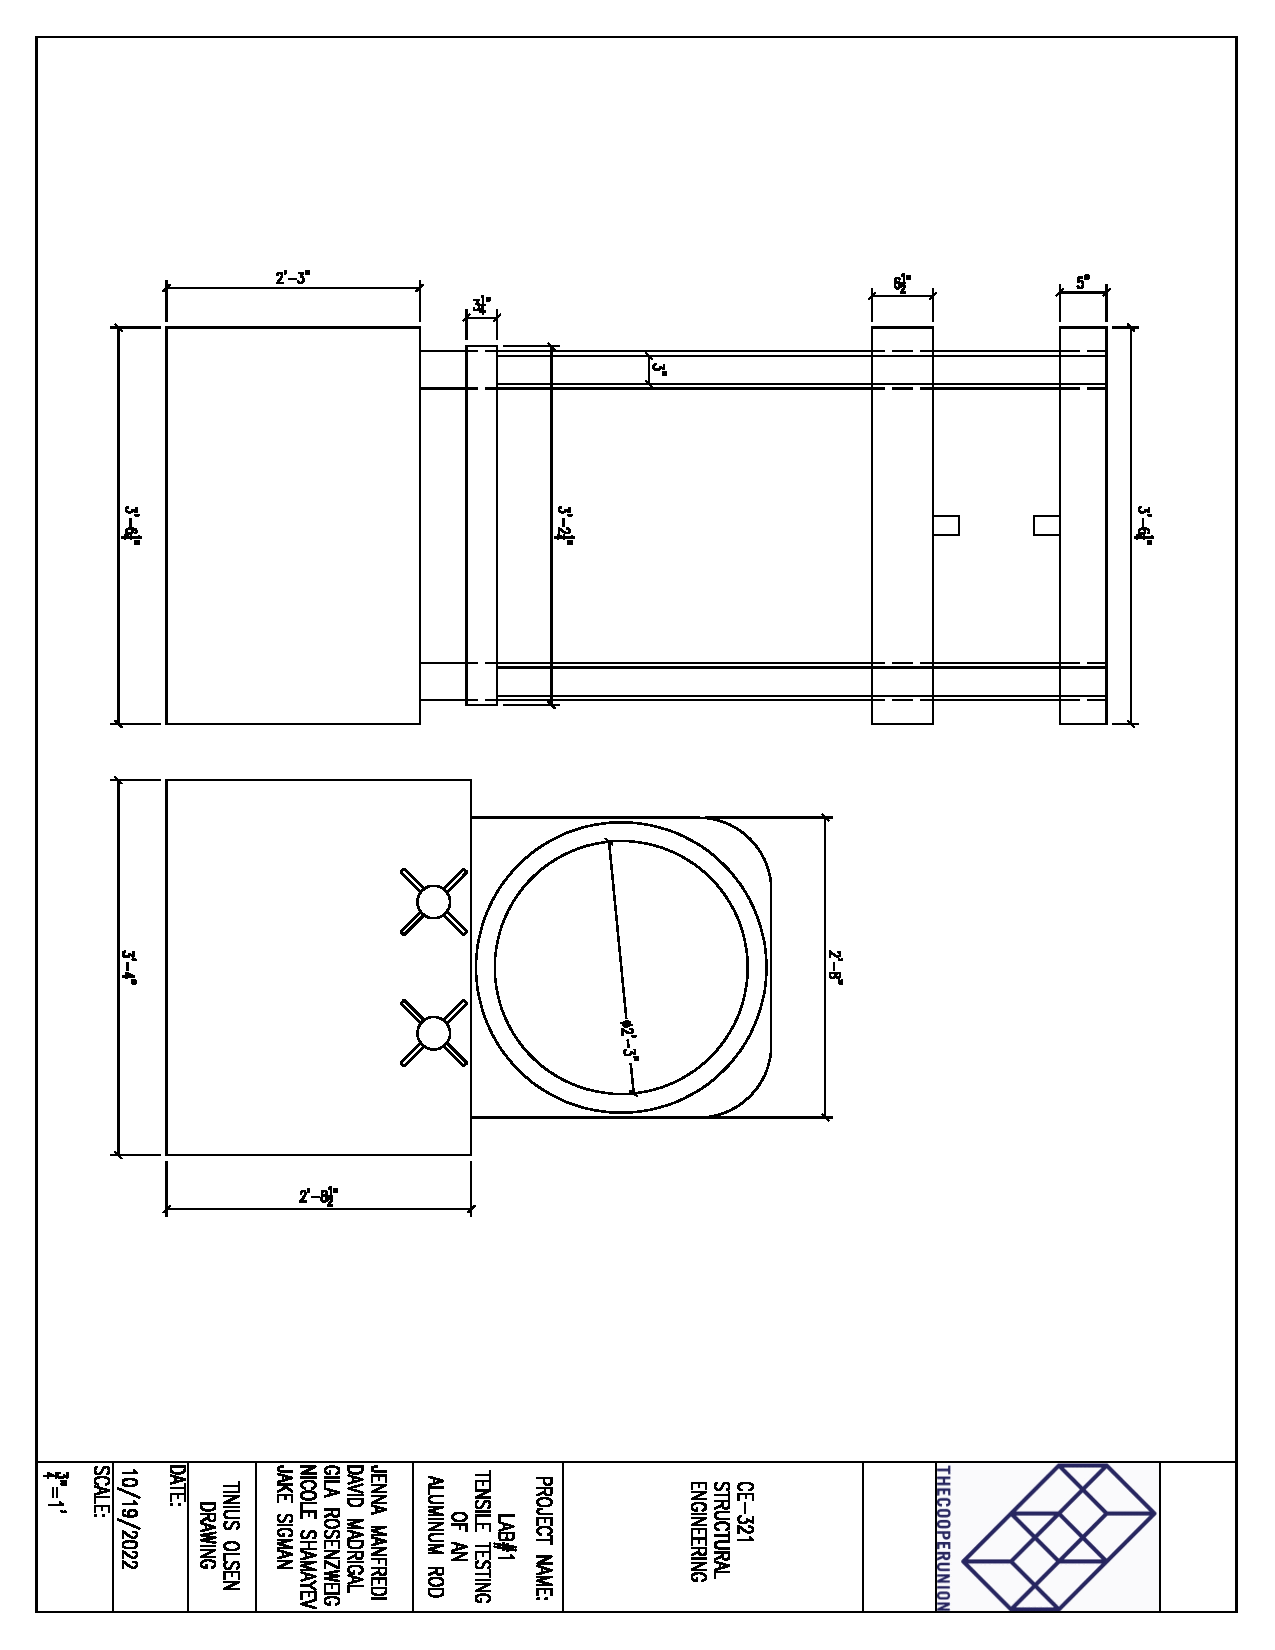
\includepdf{dwg.pdf}
    \end{center}
    \newpage
    \section{Theory}
    \noindent When an axial load is applied to a member, the stress $\sigma$ at a specific point in the member is defined by the magnitude of the load $P$ divided by the cross-sectional area $A_{0}$ at the point in question. 
	\begin{equation}
	    \sigma = \frac{P}{A_{0}}
	\end{equation}
	Similarly, a member under a tensile loading will experience a deflection $\delta$; the percent change in the original length $L_{0}$ of the member is defined as the strain $\epsilon$. 
    \begin{equation}
        \epsilon = \frac{\delta}{L_{0}}
    \end{equation}
    Different materials will experience higher or lower deflections at a given load. When the relationship between stress and strain is linear, Hooke's Law applies: 
    \begin{equation}
        \sigma = E \epsilon 
    \end{equation}
    where E is defined as the \emph{modulus of elasticity} or \emph{Young's modulus} of the material. \\\\Equation 3 is significant as it defines the elastic region of the stress-strain curve; materials undergoing loading will exhibit elastic deformation when Hooke's Law holds. The \emph{proportional limit} of a material is defined as the point where equation 3 no longer holds. This is in contrast to the \emph{yield strength $\sigma_{y}$}, which is the point where permanent set begins. For this laboratory experiment it is assumed that the differences between the proportional limit and yield strength are negligible due to the ductility of metals, and are therefore the same.\\\\
    Equations 1 and 2 can be substituted into equation 3 to get a direct relationship between the load applied and the deflection observed:
    \[\sigma = E \epsilon \Rightarrow \frac{P}{A_{0}} = E \frac{\delta}{L_{0}}\]
    \begin{equation}
        \delta = \frac{P L_{0}}{A_{0} E}
    \end{equation}
    This equation is especially useful as the input quantities for length, cross-sectional area, and modulus of elasticity can be determined from simple measurements.\\\\
    When the yield strength is reached, the material experiences permanent offset. This means that when the member  is unloaded, it does not return to its original length and thus has been permanently deformed. The permanent offset is also known as \emph{plastic deformation} and once the yield strength is reached the member is said to deform plastically. Hooke's Law as expressed by equations 3 and 4 do not hold in the plastic region of a material. When a ductile material undergoes plastic deformation, it will experience much larger deformation with smaller increases in the load. Eventually, the \emph{ultimate tensile strength $\sigma_{u}$} is reached; this is the maximum load the material can take. Once the ultimate strength is reached, a phenomena can be observed where the cross-sectional area of the member at a point will decrease; this is known as \emph{necking}, and lower loads are sufficient to cause deformation. Rupture occurs when the member can no longer take any stresses. The stress at rupture is defined as the \emph{breaking stress $\sigma_{b}$}.\\\\
    Equations 1 and 2 define the \emph{engineering} stress and strain of a material undergoing axial loading. However, this consideration only takes into account the original length $L_{0}$ and original cross-sectional area $A_{0}$, and not the fact that the length and cross-sectional area of the members changes with loading. Thus, a more accurate measure for stress and strain accounts for these changes; this is known as \emph{true stress $\sigma_{t}$ } and \emph{true strain $\epsilon_{t}$ } For true stress:
    \begin{equation}
        \sigma_{t} = \frac{P}{A} 
    \end{equation}
    where $A$ is the cross-sectional area of the member at the specific loading. For true strain, every recorded length for every specific loading is considered as an integral:
    \begin{equation}
        \epsilon_{t} = \int_{L_{0}}^{L}\frac{dL}{L}\
    \end{equation}
    where $L$ is the length of the member at a specific loading. The true stress and true strain are a more accurate measure than the engineering stress; however, they will not be used in this experiment as the cross-sectional area changes cannot be determined by simple measurement. \\\\
    The stress-strain curves for a material undergoing  tensile loading are highly relevant to structural engineering, primarily for the determination of the yield strength of a specific member to prevent plastic deformation. However, the yield strength must never be reached and therefore safety factors must be introduced to prevent yielding, which lends itself to two crucial methodologies of structural design (Load and Resistance Factor Design vs Allowable Stress Design). Thus, the material properties determined by a tensile test (and by extension a compression test) are invaluable to structural design.
    \newpage
    \section{Sample Calculations}
    \subsection{Cross-Sectional Area}
    \[A=\frac{\pi}{4}\times d^2\]
    \[A=\frac{\pi}{4}\times (0.505\text{ in})^2=\boxed{0.2\text{ in}^2}\]
    \subsection{Stress}
    \[\sigma=\frac{P}{A}\]
    \[\sigma=\frac{11500\text{ lb}}{0.2\text{ in}^2}=\boxed{57500\text{ psi}}\]
    \subsection{Strain}
    \[\varepsilon=\frac{\delta}{L}\]
    \[\varepsilon=\frac{0.143\text{ in}}{4.519\text{ in}}=\boxed{0.0316}\]
    \subsection{Modulus of Elasticity}
    \[E=\frac{P\times L}{A\times \delta}\]
    \[E=\frac{11500\text{ lb}\times 4.519\text{ in}}{0.2\text{ in}^2\times (0.143\text{ in}-0.101\text{ in})}=\boxed{6177578\text{ psi}}\]
    \subsection{Error}
    \[\%_\text{Error}=\frac{|\text{Theoretical}-\text{Experimental}|}{\text{Theoretical}}\times 100\%\]
    \[\%_\text{Error}=\frac{|\text{10600000 psi}-\text{6177578 psi}|}{\text{10600000 psi}}\times 100\%=\boxed{41.72\%}\]
    \newpage
    \section{Results}
    \begin{center}
    \addcontentsline{lot}{table}{Table 1: Measured and Observed Data}
    {\large{\bf Table 1: Measured and Observed Data\\}}
    \vspace{3mm}
    \begin{tabular}{| l r | l r |}
        \hline
        \multicolumn{2}{|c|}{\textbf{Measured}} & \multicolumn{2}{|c|}{\textbf{Observed}} \\ \hline
        Diameter & 0.505 in & Yield Deflection & 0.102 in \\
        Rod Length & 4.519 in & Yield Force & 10500 lbs \\
        Inner Rod Length & 2.45 in & Ultimate Yield Force & 13500 lbs \\ \hline
    \end{tabular}
    \vspace{10mm}
    \addcontentsline{lot}{table}{Table 2: Experimental and Theoretical Results}
    {\large{\bf \\Table 2: Experimental and Theoretical Results\\}}
    \vspace{3mm}
    \begin{tabular}{|l | l r |}
        \hline
        \multirow{2}{*}{\textbf{Modulus of Elasticity}} & Theoretical & 10600 ksi\\
        & Experimental & 6177.58 ksi \\\hline
        \multirow{2}{*}{\textbf{Ultimate Tensile Strength}} & Theoretical & 68000 psi\\
        & Experimental & 67400.19 psi \\\hline
        \multirow{2}{*}{\textbf{Proportional Limit}} & Theoretical & 47000 psi\\
        & Experimental & 52000 psi \\\hline
    \end{tabular}
    \vspace{10 mm}
    \addcontentsline{lot}{table}{Table 3: Initial Loading}
    {\large{\bf \\Table 3: Initial Loading\\}}
    \vspace{3mm}
    \begin{tabular}{|c c c c||c c c c|}
        \hline
        \textbf{P (lb)} & \(\bm{\delta}\)\textbf{ (in)} & \(\bm{\sigma}\)\textbf{ (psi)} & \(\bm{\varepsilon}\) & \textbf{P (lb)} & \(\bm{\delta}\)\textbf{ (in)} & \(\bm{\sigma}\)\textbf{ (psi)} & \(\bm{\varepsilon}\)\\ \hline
        0 & 0.000 & 0.0000 & 0.0000 & 6000 & 0.039 & 29955.6407 & 0.0086\\ 
        500 & 0.005 & 2496.3034 & 0.0011 & 6500 & 0.044 & 32451.9441 & 0.0097\\ 
        1000 & 0.008 & 4992.6068 & 0.0018 & 7000 & 0.048 & 34948.2475 & 0.0106\\ 
        1500 & 0.011 & 7488.9102 & 0.0024 & 7500 & 0.053 & 37444.5509 & 0.0117\\ 
        2000 & 0.015 & 9985.2136 & 0.0033 & 8000 & 0.058 & 39940.8543 & 0.0128\\ 
        2500 & 0.017 & 12481.5170 & 0.0038 & 8500 & 0.063 & 42437.1577 & 0.0139\\ 
        3000 & 0.019 & 14977.8203 & 0.0042 & 9000 & 0.068 & 44933.4610 & 0.0150\\ 
        3500 & 0.021 & 17474.1237 & 0.0046 & 9500 & 0.072 & 47429.7644 & 0.0159\\ 
        4000 & 0.023 & 19970.4271 & 0.0051 & 10000 & 0.078 & 49926.0678 & 0.0173\\ 
        4500 & 0.025 & 22466.7305 & 0.0055 & 10500 & 0.102 & 52422.3712 & 0.0226\\ 
        5000 & 0.029 & 24963.0339 & 0.0064 & 10750 & 0.115 & 53670.5229 & 0.0254\\ 
        5500 & 0.034 & 27459.3373 & 0.0075 & 11000 & 0.124 & 54918.6746 & 0.0274\\ \hline
    \end{tabular}
    \newpage
    \addcontentsline{lot}{table}{Table 4: Unloading}
    {\large{\bf Table 4: Unloading\\}}
    \vspace{3mm}
    \begin{tabular}{|c c c c||c c c c|}
        \hline
        \textbf{P (lb)} & \(\bm{\delta}\)\textbf{ (in)} & \(\bm{\sigma}\)\textbf{ (psi)} & \(\bm{\varepsilon}\) & \textbf{P (lb)} & \(\bm{\delta}\)\textbf{ (in)} & \(\bm{\sigma}\)\textbf{ (psi)} & \(\bm{\varepsilon}\) \\ \hline
        10500 & 0.138 & 52422.3712 & 0.0305 & 5000 & 0.124 & 24963.0339 & 0.0274 \\
        10000 & 0.137 & 49926.0678 & 0.0303 & 4500 & 0.123 & 22466.7305 & 0.0272 \\ 
        9500 & 0.136 & 47429.7644 & 0.0301 &4000 & 0.121 & 19970.4271 & 0.0268 \\ 
        9000 & 0.134 & 44933.4610 & 0.0297 &3500 & 0.12 & 17474.1237 & 0.0266 \\ 
        8500 & 0.133 & 42437.1577 & 0.0294 &3000 & 0.118 & 14977.8203 & 0.0261 \\ 
        8000 & 0.132 & 39940.8543 & 0.0292 &2500 & 0.116 & 12481.5170 & 0.0257 \\
        7500 & 0.131 & 37444.5509 & 0.0290 &2000 & 0.114 & 9985.2136 & 0.0252 \\ 
        7000 & 0.129 & 34948.2475 & 0.0285 &1500 & 0.112 & 7488.9102 & 0.0248 \\
        6500 & 0.128 & 32451.9441 & 0.0283 &1000 & 0.108 & 4992.6068 & 0.0239 \\ 
        6000 & 0.127 & 29955.6407 & 0.0281 &500 & 0.103 & 2496.3034 & 0.0228 \\ 
        5500 & 0.125 & 27459.3373 & 0.0277 &0 & 0.056 & 0.0000 & 0.0124 \\ \hline        
    \end{tabular}
    \vspace{5 mm}
    \addcontentsline{lot}{table}{Table 5: Reloading}
    {\large{\bf \\Table 5: Reloading\\}}
    \vspace{3mm}
    \begin{tabular}{|c c c c || c c c c|}
        \hline
        \textbf{P (lb)} & \(\bm{\delta}\)\textbf{ (in)} & \(\bm{\sigma}\)\textbf{ (psi)} & \(\bm{\varepsilon}\) & \textbf{P (lb)} & \(\bm{\delta}\)\textbf{ (in)} & \(\bm{\sigma}\)\textbf{ (psi)} & \(\bm{\varepsilon}\) \\ \hline
        0 & 0.056 & 0.0000 & 0.0124 &7000 & 0.126 & 34948.2475 & 0.0279 \\ 
        500 & 0.101 & 2496.3034 & 0.0224 &7500 & 0.127 & 37444.5509 & 0.0281 \\ 
        1000 & 0.104 & 4992.6068 & 0.0230 &8000 & 0.128 & 39940.8543 & 0.0283 \\ 
        1500 & 0.106 & 7488.9102 & 0.0235 &8500 & 0.13 & 42437.1577 & 0.0288 \\ 
        2000 & 0.11 & 9985.2136 & 0.0243 &9000 & 0.132 & 44933.4610 & 0.0292 \\ 
        2500 & 0.112 & 12481.5170 & 0.0248 &9500 & 0.133 & 47429.7644 & 0.0294 \\ 
        3000 & 0.114 & 14977.8203 & 0.0252 &10000 & 0.135 & 49926.0678 & 0.0299 \\ 
        3500 & 0.115 & 17474.1237 & 0.0254 &10500 & 0.136 & 52422.3712 & 0.0301 \\ 
        4000 & 0.117 & 19970.4271 & 0.0259 &11000 & 0.139 & 54918.6746 & 0.0308 \\ 
        4500 & 0.118 & 22466.7305 & 0.0261 &11500 & 0.143 & 57414.9780 & 0.0316 \\ 
        5000 & 0.12 & 24963.0339 & 0.0266 &12000 & 0.192 & 59911.2814 & 0.0425 \\ 
        5500 & 0.121 & 27459.3373 & 0.0268 &12500 & 0.224 & 62407.5848 & 0.0496 \\ 
        6000 & 0.123 & 29955.6407 & 0.0272 &13000 & 0.295 & 64903.8882 & 0.0653 \\ 
        6500 & 0.124 & 32451.9441 & 0.0274 &13500 & 0.4 & 67400.1916 & 0.0885 \\ \hline         
    \end{tabular}
    \newpage
    \addcontentsline{lot}{table}{Table 6: Theoretical Data}
    \begin{center}
        \doublespacing
    {\large{\bf Table 6: Theoretical Data\\}}
    \vspace{3mm}
    \begin{tabular}{|c c c c||c c c c|}
        \hline
        \textbf{P (lb)} & \(\bm{\delta}\)\textbf{ (in)} & \(\bm{\sigma}\)\textbf{ (psi)} & \(\bm{\varepsilon}\) & \textbf{P (lb)} & \(\bm{\delta}\)\textbf{ (in)} & \(\bm{\sigma}\)\textbf{ (psi)} & \(\bm{\varepsilon}\) \\ \hline
        0     & 0        & 0        & 0           &7000  & 0.014899 & 34948.25 & 0.003297004 \\
        500   & 0.001064 & 2496.303 & 0.0002355   &7500  & 0.015963 & 37444.55 & 0.003532505 \\
        1000  & 0.002128 & 4992.607 & 0.000471001 &8000  & 0.017028 & 39940.85 & 0.003768005 \\
        1500  & 0.003193 & 7488.91  & 0.000706501 &8500  & 0.018092 & 42437.16 & 0.004003505 \\
        2000  & 0.004257 & 9985.214 & 0.000942001 &9000  & 0.019156 & 44933.46 & 0.004239006 \\
        2500  & 0.005321 & 12481.52 & 0.001177502 &9500  & 0.02022  & 47429.76 & 0.004474506 \\
        3000  & 0.006385 & 14977.82 & 0.001413002 &10000 & 0.021285 & 49926.07 & 0.004710006 \\
        3500  & 0.00745  & 17474.12 & 0.001648502 &10500 & 0.022349 & 52422.37 & 0.004945507 \\
        4000  & 0.008514 & 19970.43 & 0.001884003 &11000 & 0.023413 & 54918.67 & 0.005181007 \\
        4500  & 0.009578 & 22466.73 & 0.002119503 &11500 & 0.024477 & 57414.98 & 0.005416507 \\
        5000  & 0.010642 & 24963.03 & 0.002355003 &12000 & 0.025541 & 59911.28 & 0.005652008 \\
        5500  & 0.011706 & 27459.34 & 0.002590504 &12500 & 0.026606 & 62407.58 & 0.005887508 \\
        6000  & 0.012771 & 29955.64 & 0.002826004 &13000 & 0.02767  & 64903.89 & 0.006123008 \\
        6500  & 0.013835 & 32451.94 & 0.003061504 &13500 & 0.028734 & 67400.19 & 0.006358509 \\\hline
    \end{tabular}
\end{center}
\end{center}
\newpage
\begin{center}
    \doublespacing
        \begin{tikzpicture}[baseline=(current bounding box.center)]
            \addcontentsline{lof}{figure}{Figure 1: Stress vs. Strain Curve}
            \begin{axis}[
                title={\textbf{Figure 1: Stress vs. Strain Curve}},
                xlabel={\(\varepsilon\)},
                ylabel={\(\sigma\) (psi)},
                ymin=0, ymax=90000,
                xmin=0, xmax=0.09,
                xticklabel style={
                /pgf/number format/precision=3,
                /pgf/number format/fixed},
                ytick={0,10000,20000,30000,40000,50000,60000,70000,80000,90000},
                xtick={0,0.01,0.02,0.03,0.04,0.05,0.06,0.07,0.08,0.09},
                ymajorgrids=true,
                grid style=dashed,
                cells={anchor=west},
                width=0.9\textwidth,
                height=1.3\textwidth
            ]
            
            \addplot[smooth, red] table [x=strain, y=stress] {fig1.csv};
            \addplot[smooth, orange, domain=0:0.004433962] {10600000*x};
            \addplot[smooth, orange, domain=0.004433962:0.1] {113167.2598*x+46498.22064};
            \addlegendentry{Experimental}
            \addlegendentry{Theoretical}
            \end{axis}
        \end{tikzpicture}
    \end{center}
    \newpage
    \begin{center}
        \begin{tikzpicture}[baseline=(current bounding box.center)]
            \addcontentsline{lof}{figure}{Figure 2: Experimental Stress vs. Strain Curve}
            \begin{axis}[
                title={\textbf{Figure 2: Experimental Stress vs. Strain Curve}},
                xlabel={\(\varepsilon\)},
                ylabel={\(\sigma\) (psi)},
                ymin=0, ymax=90000,
                xmin=0, xmax=0.09,
                xticklabel style={
                /pgf/number format/precision=3,
                /pgf/number format/fixed},
                ytick={0,10000,20000,30000,40000,50000,60000,70000,80000,90000},
                xtick={0,0.01,0.02,0.03,0.04,0.05,0.06,0.07,0.08,0.09},
                ymajorgrids=true,
                grid style=dashed,
                cells={anchor=west},
                width=0.9\textwidth,
                height=1.3\textwidth
            ]
            
            \addplot[no markers, blue, dashed, domain=0:0.07] {1814394*x-1814.39};
            \addplot[no markers, purple, dashed, domain=0:0.07] {1814394*x-9071.97};
            \addplot[smooth, red] table [x=strain, y=stress] {fig1.csv};
            \addlegendentry{0.1\% Offset}
            \addlegendentry{0.5\% Offset}
            \end{axis}
        \end{tikzpicture}
    \end{center}
    \newpage
    \begin{center}
        \begin{tikzpicture}[baseline=(current bounding box.center)]
            \addcontentsline{lof}{figure}{Figure 3: Theoretical Stress vs. Strain Curve}
            \begin{axis}[
                title={\textbf{Figure 3: Theoretical Stress vs. Strain Curve}},
                xlabel={\(\varepsilon\)},
                ylabel={\(\sigma\) (psi)},
                ymin=0, ymax=70000,
                xmin=0, xmax=0.09,
                xticklabel style={
                /pgf/number format/precision=3,
                /pgf/number format/fixed},
                ytick={0,10000,20000,30000,40000,50000,60000,70000},
                xtick={0,0.01,0.02,0.03,0.04,0.05,0.06,0.07,0.08,0.09},
                ymajorgrids=true,
                grid style=dashed,
                cells={anchor=west},
                width=0.9\textwidth,
                height=1.3\textwidth
            ]
            
            \addplot[smooth, orange, domain=0:0.004433962] {10600000*x};
            \addplot[no markers, blue, dashed, domain=0:0.07] {10600000*x-10600};
            \addplot[no markers, purple, dashed, domain=0:0.07] {10600000*x-53000};
            \addplot[smooth, orange, domain=0.004433962:0.1] {113167.2598*x+46498.22064};
            \addlegendentry{Theoretical}
            \addlegendentry{0.1\% Offset}
            \addlegendentry{0.5\% Offset}
            \end{axis}
        \end{tikzpicture}
    \end{center}
    \newpage
    \section{Conclusion}
    \indent Tensile properties of a material are best characterized by subjecting a material specimen to tensile forces in a controlled testing environment. Material tensile properties carry significant importance in engineering design considerations; loads exceeding the yield strength of material cause permanent deflections and eventually failure and as such must be chosen particularly for the intended use.  \\
    \indent There are several variables that can affect tensile strengths of aluminum alloys: alloy composition, casting conditions, heat treatment, geometry of specimens, and test conditions some of those variables. There are other experiments and research that analyze and compare tensile properties considering the effects of alloying and heat treatment, and still others that consider casting conditions and alloy compositions. Such experiments are useful in determining the best casting methods and allow compositions. This experiment used a single specimen, with the intent of comparing experimental values to theoretical values for the same metrics. The tensile test conducted placed a specimen of known dimensions between clamps, and keeping one end fixed, load (force) is applied to the material at the other end; the load is increased and the change in length of the sample is measured. Using these data, both engineering stress and strain is calculated, and the relation between the two determines the Youngs’ modulus of the material. Youngs’ modulus can be used to compare strengths between different materials; a stress-strain curve as displayed above is a simple method for comparing materials. Loading a specimen to breaking point allows one to determine both elastic and plastic tensile deformation properties.  \\
    \indent Looking at the graphs produced from the experimental data, the T351 sample was observed as yielding at approximately 10,500 lbs in the initial loading, and between 9,000 and 10,000 lbs in the reloading. For calculating yield strength (stress), more accurate results are obtained by using data from the reloading; the reason for this is because there was some observable slipping at the start of the initial loading. At 9,000 lbs of load the calculated stress is 45,000 psi, at 9,500 lbs the calculated stress is 47,500 psi, and at 10,000 lbs the stress is 50,000 psi. Because it is difficult to tell precisely where yielding began, it is reasonable to assume that 9,500 lbs is the approximate load above which plastic deformation begins. Failure occurred at approximately 13,500 lbs, giving a calculated ultimate tensile strength of 67,500 psi.  \\
    \indent The expected maximum load before yield was determined as 9,400 lbs, using the theoretical yield stress of 47,000 psi and the calculated cross-sectional area of 0.2 \(\text{in}^2\). Theoretical ultimate tensile strength is published as 68,000 psi. The calculated values for tensile yield strength, maximum load before yielding, and ultimate tensile strengths are reasonably close to the theoretical values: the percent error for tensile yield strength was 1.06\%, for ultimate yield strength 0.88\%, and for the 0.1\% and 0.5\% offset yield strengths, percent error was 23.4\% and 22.9\% respectively. The observed yield load was 100 lbs greater than the theoretical yield load. The experimental yield strength was 500 lbs greater than the theoretical yield strength. Experimental ultimate tensile strength was 500 lbs below the theoretical value. In all calculated values, including maximum load before yielding, and stress (strength) values, error is introduced from instrumental error of the Vernier calipers used to determine the cross-sectional diameter of the specimen. In stress calculations, error is introduced from procedural errors: data points were recorded at approximately every 500 lbs, which is subject to instrumental error in readings and human error by way of delay in calling the load values. Additionally, because data was recorded at increments of 500 lbs, if critical loading is at some point not in increments of 500, the yield point will not be read with complete accuracy, and the experimental yield stress will thus be different as well.  \\
    \indent Deformation of the specimen was calculated at every data point; there was a permanent deformation at the end of the unloading stage of 0.056 in; this is due to the fact that the initial loading was not stopped at the precise point of yield, and was instead stopped at 11,000 lbs. Graphically, this results in the reloading curve being offset from the initial load curve. Engineering strain is calculated as a ratio of the deformation to original length; at the observed yield load of 9,500 lbs, the theoretical strain is 0.00447, and the calculated experimental strain is 0.0294. The discrepancy in strain value is due to the deformations being larger experimentally than theoretically. There are several reasons the deformations may be large: human/procedural error, instrumental error, different temperature conditions, slipping of the rod between the grips. To discuss these individually, an error in the readings may have occurred due to the fact that there is a delay between the load being called out, and the deformation being called and read; there is also instrumental error in reading the deformations, as there is a limit on the precision of the instrument. Different temperature conditions make a material more and less ductile – if the experiment conditions were warm, the material may have experienced more ductility and thus more deformation than otherwise. Lastly, there was noticeable slipping at the start of the loading procedure, which resulted in load being applied without deformation occurring; it is not unreasonable to assume there might have been slipping, though unnoticeable in observation, during the reloading procedure. The discrepancy in deformation values leads to strain values such that the modulus of elasticity will be different as well. This is reflected in the percent error of 41.72\%.  \\
    \indent The specimen failed at values very close to the theoretical values, indicating that the theoretical values hold. The modulus of elasticity was calculated at a value much smaller than the theoretical; this can be attributed to error as described above. Graphically, the experimental modulus of elasticity (slope of the linear portion of the stress-strain curve) looks to be approximately equal to the theoretical value; this is due to the scaling of the graph. To improve this experiment, the area of concern should be the deformations; it would be wise to take measures to ensure little to no slippage during loading.  
    \newpage
    \section{References}
    \begin{description}
        
        \item Lars, A. \emph{et. al.} (2017). Evaluating the Tensile Properties of Aluminum Foundry Alloys through Reference Castings-A Review, \url{https://pubmed.ncbi.nlm.nih.gov/28867796/} (accessed 16 October 2022).
        \item Ferdinand B. \emph{et. al.} (2015). \emph{Mechanics of Materials}, 7th Ed., McGraw Hill, New York.
        \item Fahmi, M. \emph{et. al.} (2009). Influence of specimen preparation, microstructure anisotropy, and residual stresses on stress–strain curves of rolled Al2024 T351 as derived from spherical indentation tests, \url{https://www.researchgate.net/publication/231791029_Influence_of_specimen_preparation_microstructure_anisotropy_and_residual_stresses_on_stress-strain_curves_of_rolled_Al2024_T351_as_derived_from_spherical_indentation_tests} (accessed 16 October 2022).
        \item ASM Material Data Sheet - Aluminum 2024-T4; 2024-T351, \url{https://asm.matweb.com/search/SpecificMaterial.asp?bassnum=ma2024t4} (accessed 16 October 2022).
        \item Engineering Archives - Offset Yield Method, \url{http://www.engineeringarchives.com/les_mom_offsetyieldmethod.html} (accessed 16 October 2022).
        \item Michigan Technological University - Tensile Test Experiment, \url{https://www.mtu.edu/materials/k12/experiments/tensile/} (accessed 16 October 2022).
        
    \end{description}
    \newpage
    \section{Appendix}
    \begin{center}
    \noindent Rod Diameter, D (in): 0.505\\
    Rod Length, L (in): 4.519 \\
    Inner Rod Length, \(\text{L}_\text{inner}\) (in): 2.45 \\
    Rod Cross-Sectional Area, A \(\left(\text{in}^2\right)\): 0.2 \\
    \end{center}
    \begin{center}
        \begin{tabular}{|l c c|}
            \hline
            & \textbf{Theoretical} & \textbf{Experimental} \\\hline
            Modulus of Elasticity, E (psi) & 10600000 & 6177578\\
            Proportional Limit, \(\sigma_\text{PL}\) (psi) & 47000 & 47500\\
            0.1\% Offset Yield Strength, \(\sigma_\text{y0.1\%}\) (psi) & 47000 & 58000\\
            0.5\% Offset Yield Strength, \(\sigma_\text{y0.5\%}\) (psi) & 48000 & 59000\\
            Ultimate Tensile Strength, \(\sigma_\text{UTS}\) (psi) & 68000 & 67400.19\\\hline 
        \end{tabular}
        \vspace{2mm}
    \end{center}
    \begin{center}
        Modulus of Elasticity Percentage Error, Error E (\%): 41.72 \\
        Proportional Limit Percentage Error, Error \(\sigma_\text{PL}\) (\%): 1.06\\
        0.1\% Offset Yield Strength, Error \(\sigma_\text{y0.1\%}\) (\%): 23.4\\
        0.5\% Offset Yield Strength, Error \(\sigma_\text{y0.5\%}\) (\%): 22.9\\
        Ultimate Tensile Strength, Error \(\sigma_\text{UTS}\) (\%): 0.88\\
    \end{center}
\end{document}